\newcommand{\vE}{\vb{E}}
\newcommand{\vS}{\vb{S}}
\newcommand{\vSA}{\vS^A}
\newcommand{\vSB}{\vS^B}
\newcommand{\Max}{\text{Max}}
\newcommand{\kpsi}{\ket{\psi}}
\newcommand{\up}{\uparrow}
\newcommand{\dn}{\downarrow}
\newcommand{\kupz}{\ket{\up_z}}
\newcommand{\kdnz}{\ket{\dn_z}}
\newcommand{\Sx}{S_x}
\newcommand{\Sz}{S_z}
\newcommand{\SxA}{\Sx^A}
\newcommand{\SzA}{\Sz^A}
\newcommand{\SxB}{\Sx^B}
\newcommand{\SzB}{\Sz^B}
\newcommand{\dhf}{\dfrac{1}{2}}

\begin{statement}{}
	Consider the following probabilistic game: There are four doors ($Q, R, S, T$).  Behind each door is a device which displays $\pm 1$ randomly according to the probability $P(Q=\pm1, R=\pm1, S=\pm1, T=\pm1)$.  Alice and Bob are on the same team.  Alice has to choose either $Q$ and $R$, and then Bob has to choose either $S$ and $T$.  When the numbers match, they get $+1$ point; when the numbers do not match, they get $-1$ point.  However, when they open $Q$ and $T$, it's an exception.  When the numbers (do not) match, they get $-1$~($+1$).
\end{statement}

\begin{problem} \label{1.1}
	Let's assume Alice and Bob open the doors completely randomly.  When all numbers are $+1$ with probability 1, what is the expectation value of the point they get?
\end{problem}

\begin{solution}
	Let $\vE$ be the expectation value of the number of points.  In this case, the numbers behind the two doors will always match.  So
	\beq
		\vE = \frac{QS + RS + RT - QT}{4}
		= \frac{1 + 1 + 1 - 1}{4}
		= \frac{1}{2}.
	\eeq
	\vfix
\end{solution}



\begin{problem}
	As it turns out, irrespective of how hard you fine tune the probability $P(Q=\pm1, R=\pm1, S=\pm1, T=\pm1)$, the expectation value of the point Alice and Bob get cannot exceed a certain value $\Max$:
	\beq
		\frac{\vE(QS) + \vE(RS) + \vE(RT) - \vE(QT)}{4} \leq \Max.
	\eeq
	Here, $\vE(QS)$, etc. is the expectation value of the point when Alice opens $Q$ and Bob opens $S$.  This is a Bell inequality.  Determine $\Max$.
	
	\emph{Hint:} For a given realization of the numbers $Q = \pm1$, $R = \pm1$, $S = \pm1$, $T = \pm1$, which occurs with probability $P(Q, R, S, T)$, note that $QS + RS + RT - QT = (Q+R)S + (R-Q)T$, where one of $\{(R+Q), (R-Q)\}$ is 2 and the other 0.
\end{problem}

\begin{solution}
	In addition to the information provided in the hint, both $S$ and $T$ must be $\pm1$.  This means the only possibilities for the number of points earned are
	\beq
		\frac{(Q + R) S + (R - Q) T}{4} = \begin{cases}
			\dfrac{(0) (-1) + (2) (1)}{4} = \dfrac{1}{2}, \\[2ex]
			\dfrac{(0) (1) + (2) (-1)}{4} = -\dfrac{1}{2}.
		\end{cases}
	\eeq
	Thus,
	\beq
		\Max = \frac{1}{2}.
	\eeq
	\vfix
\end{solution}



\begin{problem}
	Frustrated by the upper bound set by the Bell inequality, Bob decides to cheat.  He now changes the value of $T$ after Alice chooses $Q$ or $R$.  Assume $Q,R,S$ are set to be $+1$ with probability 1.  To make the expectation value of the point they get equal to $+1$, what values should Bob set after Alice chooses $Q$ or $R$?
\end{problem}

\begin{solution}
	If Alice chooses $R$, Bob should set $T = 1$.  If Alice chooses $Q$, Bob should set $T = -1$.  This way,
	\beq
		\frac{\vE(QS) + \vE(RS) + \vE(RT) - \vE(QT)}{4}
		= \frac{1 + 1 + 1 + 1}{4}
		= 1.
	\eeq
	\vfix
\end{solution}



\newcommand{\kQp}{\ket{Q_+}}
\newcommand{\kQm}{\ket{Q_-}}
\newcommand{\kTp}{\ket{T_+}}
\newcommand{\kTm}{\ket{T_-}}
\newcommand{\Apm}{A_\pm}

\newcommand{\alp}{\alpha}
\newcommand{\sig}{\sigma}
\newcommand{\sigq}{\sig_1}
\newcommand{\sigw}{\sig_2}
\newcommand{\sige}{\sig_3}

\newcommand{\ah}{\vb{\hat{a}}}
\newcommand{\bh}{\vb{\hat{b}}}
\newcommand{\nh}{\vb{\hat{n}}}
%\newcommand{\vS}{\vb{S}}
\newcommand{\tht}{\theta}
\newcommand{\thtab}{\tht_{ab}}
\newcommand{\Sn}{\vS \vdot \nh}

\newcommand{\kSnp}{\ket{\Sn; +}}
\newcommand{\kSnm}{\ket{\Sn; -}}
\newcommand{\kup}{\ket{\up}}
\newcommand{\kdn}{\ket{\dn}}

\begin{problem}
	Now consider a quantum mechanical version of the game.  There are quantum states of two spin-$1/2$ degrees of freedom shared by Alice and Bob.  Alice can measure the $z$ component or $x$ components of the first spin $\vSA$.  (This corresponds to $Q = \pm1$ or $R = \pm1$.)  Bob can measure the $-(z+x)$ component or the $(z-x)$ component of the second spin $\vSB$.  (This corresponds to $S = \pm1$ or $T = \pm1$.)
	
	More specifically, Alice and Bob share the quantum state
	\beq
		\kpsi = \frac{\kupz \otimes \kdnz - \kdnz \otimes \kupz}{\sqrt{2}}.
	\eeq
	The operators to be measured are
	\begin{align*}
		Q &= \SzA, &
		R &= \SxA, &
		S &= -\frac{\SzB + \SxB}{\sqrt{2}}, &
		T &= \frac{\SzB - \SxB}{\sqrt{2}}.
	\end{align*}
	Let us consider the case when Alice measures $Q$ and Bob measures $T$.  Calculate the probability $P(Q, T)$ for Alice and Bob getting the measurement outcomes $(Q, T) = (\pm1, \pm1)$.
\end{problem}

\begin{solution}
	From Sakurai~(3.9.11), the probability of measuring $\vS \vdot \ah$ and $\vS \vdot \bh$ to both be positive is
	\beq
		P(\ah+; \bh+) = \frac{1}{2} \sin[2](\frac{\thtab}{2}),
	\eeq
	where $\thtab$ is the angle between the $\ah$ and $\bh$ directions.  For the other combinations, we may generalize this expression using Fig.~3.9 in Sakurai, reproduced here as Fig.~\ref{sakurai}.
	
	\begin{figure} \centering
		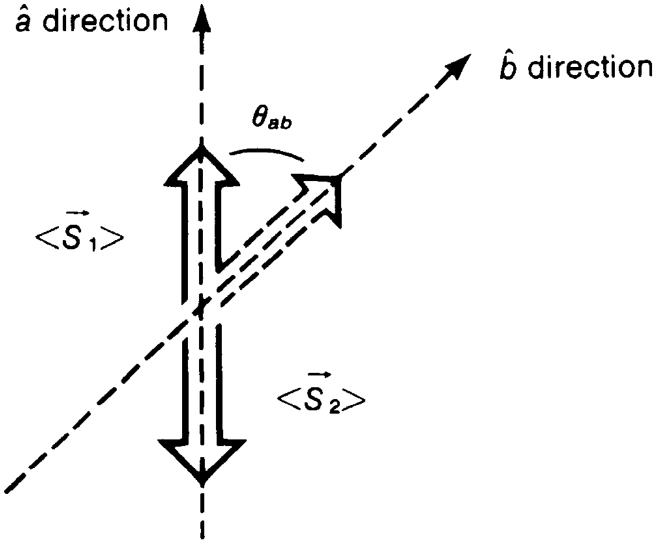
\includegraphics[width=0.4\textwidth]{3-9.jpg}
		\caption{Evaluation of $P(\ah+; \bh+)$.  Figure~3.9 in Sakurai.}
		\label{sakurai}
	\end{figure}

	This gives us
	\begin{align}
		P(\ah-; \bh-) &= \frac{1}{2} \sin[2](\frac{\thtab}{2}) = P(\ah+; \bh+), \label{prob1} \\
		P(\ah+; \bh-) &= \frac{1}{2} \sin[2](\frac{\thtab + \pi}{2}) = \frac{1}{2} \cos[2](\frac{\thtab}{2}) = P(\ah+; \bh-). \label{prob2}
	\end{align}
	For $Q$ and $T$, $\thtab = \pi / 4$.  So we have
	\begin{align*}
		P(Q=\pm1, T=\pm1) &= \frac{1}{2} \sin[2](\frac{\pi}{8})
		= \frac{1}{2} \left( \frac{\sqrt{2 - \sqrt{2}}}{2} \right)^2
		= \frac{1}{2} \frac{2 - \sqrt{2}}{4}
		= \frac{2 - \sqrt{2}}{8}
		\approx 0.073, \\
		P(Q=\pm1, T=\mp1) &= \frac{1}{2} \cos[2](\frac{\pi}{8})
		= \frac{1}{2} \left( \frac{\sqrt{2 + \sqrt{2}}}{2} \right)^2
		= \frac{1}{2} \frac{2 + \sqrt{2}}{4}
		= \frac{2 + \sqrt{2}}{8}
		\approx 0.427.
	\end{align*}
	\vfix
\end{solution}
\vspace{-2\baselineskip}


\newcommand{\kRp}{\ket{R_+}}
\newcommand{\kRm}{\ket{R_-}}
\newcommand{\kSp}{\ket{S_+}}
\newcommand{\kSm}{\ket{S_-}}

\begin{problem}
	Similarly, consider the case when Alice measures $R$ and Bob measures $T$.  Calculate the probability $P(R, T)$ for Alice and Bob getting the measurement outcomes $(R, T) = (\pm1, \pm1)$.
\end{problem}

\begin{solution}
	We can apply \refeq{prob1} and \refeq{prob2} for $R$ and $T$, where $\thtab = 3\pi / 4$.  This yields
	\begin{align*}
		P(R=\pm1, T=\pm1) &= \frac{1}{2} \sin[2](\frac{3\pi}{8})
		= \frac{1}{2} \left( \frac{\sqrt{2 + \sqrt{2}}}{2} \right)^2
		= \frac{1}{2} \frac{2 + \sqrt{2}}{4}
		= \frac{2 + \sqrt{2}}{8}
		\approx 0.427, \\
		P(R=\pm1, T=\mp1) &= \frac{1}{2} \cos[2](\frac{3\pi}{8})
		= \frac{1}{2} \left( \frac{\sqrt{2 - \sqrt{2}}}{2} \right)^2
		= \frac{1}{2} \frac{2 - \sqrt{2}}{4}
		= \frac{2 - \sqrt{2}}{8}
		\approx 0.073.
	\end{align*}
	\vfix
\end{solution}



\begin{problem}
	Compute the expectation values $\vE(QS)$, $\vE(RS)$, $\vE(QT)$, and $\vE(RT)$.  Compute
	\beq
		\frac{\vE(QS) + \vE(RS) + \vE(RT) - \vE(QT)}{4}.
	\eeq
	\vfix
\end{problem}

\begin{solution}
	We need to find the probabilities of obtaining $(Q,S) = (\pm1, \pm1)$ and $(R,S) = (\pm1, \pm1)$.  For $Q$ and $S$, $\thtab = 3\pi/4$, so another application of \refeq{prob1} and \refeq{prob2} yields
	\begin{align*}
		P(Q=\pm1, S=\pm1) &= P(R=\pm1, T=\pm1), &
		P(Q=\pm1, S=\mp1) &= P(R=\pm1, T=\mp1).
	\end{align*}
	For $R$ and $S$, $\thtab = 5\pi/4$, so
	\begin{align*}
		P(R=\pm1, S=\pm1) &= \frac{1}{2} \sin[2](\frac{5\pi}{8})
		= \frac{1}{2} \left( \frac{\sqrt{2 + \sqrt{2}}}{2} \right)^2
		= \frac{1}{2} \frac{2 + \sqrt{2}}{4}
		= \frac{2 + \sqrt{2}}{8}
		\approx 0.427, \\
		P(R=\pm1, S=\mp1) &= \frac{1}{2} \cos[2](\frac{5\pi}{8})
		= \frac{1}{2} \left( \frac{\sqrt{2 - \sqrt{2}}}{2} \right)^2
		= \frac{1}{2} \frac{2 - \sqrt{2}}{4}
		= \frac{2 - \sqrt{2}}{8}
		\approx 0.073.
	\end{align*}
	
	The expectation value of a random variable $X$ is defined
	\beq
		E(X) = \sum_{i} p_i x_i,
	\eeq
	where $x_i$ are all of the possible values of $X$, and $p_i$ the probabilities associated with each.  Then
	\begin{align*}
		\vE(QS) &= 2 P(Q=\pm1, S=\pm1) - 2 P(Q=\pm1, S=\mp1)
		= \frac{2 + \sqrt{2}}{4} - \frac{2 - \sqrt{2}}{4}
		= \frac{\sqrt{2}}{2}, \\
		\vE(RS) &= 2 P(R=\pm1, S=\pm1) - 2 P(R=\pm1, S=\mp1)
		= \frac{2 + \sqrt{2}}{4} - \frac{2 - \sqrt{2}}{4}
		= \frac{\sqrt{2}}{2}, \\
		\vE(RT) &= 2 P(R=\pm1, T=\pm1) - 2 P(R=\pm1, T=\mp1)
		= \frac{2 + \sqrt{2}}{4} - \frac{2 - \sqrt{2}}{4}
		= \frac{\sqrt{2}}{2}, \\
		\vE(QT) &= 2 P(Q=\pm1, T=\pm1) - 2 P(Q=\pm1, T=\mp1)
		= \frac{2 - \sqrt{2}}{4} - \frac{2 + \sqrt{2}}{4}
		= -\frac{\sqrt{2}}{2}.
	\end{align*}
	Finally,
	\beq
		\frac{\vE(QS) + \vE(RS) + \vE(RT) - \vE(QT)}{4}
		= \frac{1}{4} \left( \frac{\sqrt{2}}{2} + \frac{\sqrt{2}}{2} + \frac{\sqrt{2}}{2} + \frac{\sqrt{2}}{2} \right)
		= \frac{\sqrt{2}}{2},
	\eeq
	which is greater than $\Max$, thereby violating Bell's inequality.
\end{solution}